\begin{figure}[!htbp]%
    % \makebox[\textwidth][c]{
    \centering
    \begin{subfigure}[t]{0.6006\textwidth}
        \centering
        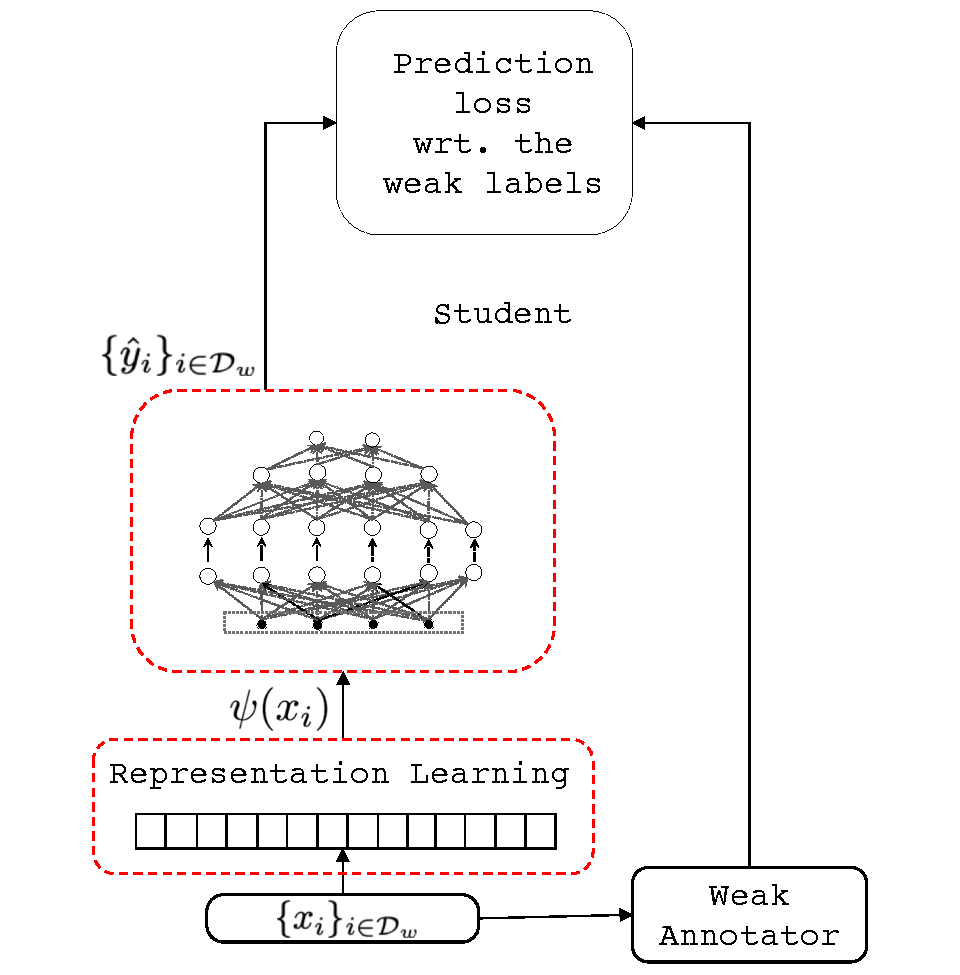
\includegraphics[width=\textwidth]{03-part-02/chapter-05/figs_and_tables/fig_fwl_step_1.pdf}
        \caption{\label{fig:step1}Step 1}
    \end{subfigure}%
    ~
    \begin{subfigure}[t]{0.462\textwidth}
        \centering
        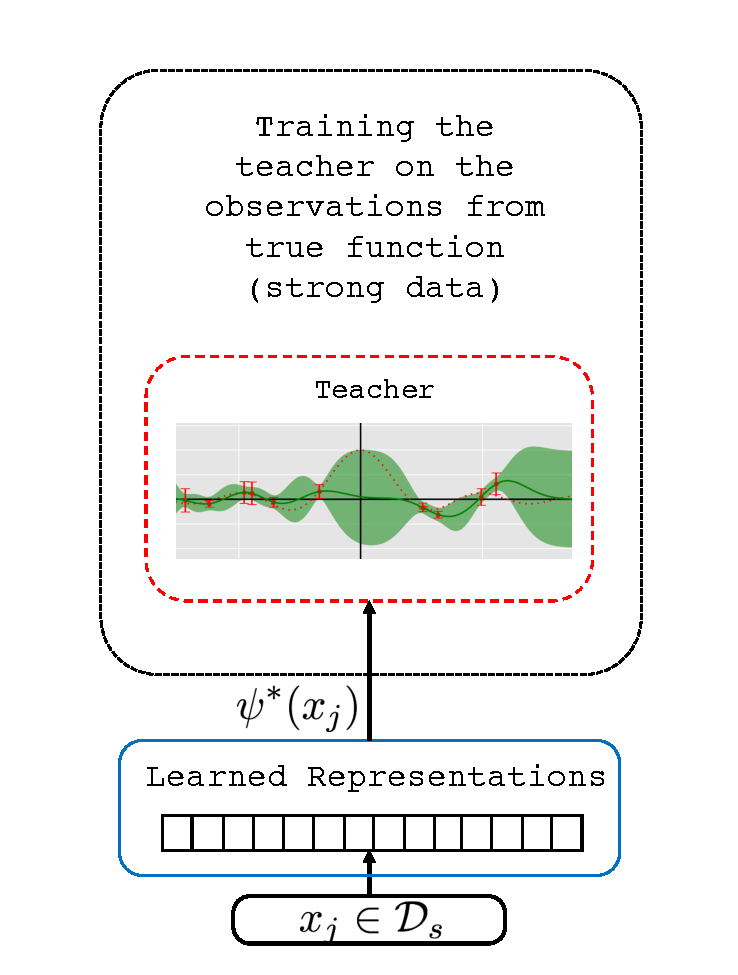
\includegraphics[width=\textwidth]{03-part-02/chapter-05/figs_and_tables/fig_fwl_step_2.pdf}
        \caption{\label{fig:step2}Step 2}
    \end{subfigure}%
    \vfill
    \vspace{30pt}
    \begin{subfigure}[t]{0.7854\textwidth}
        \centering
        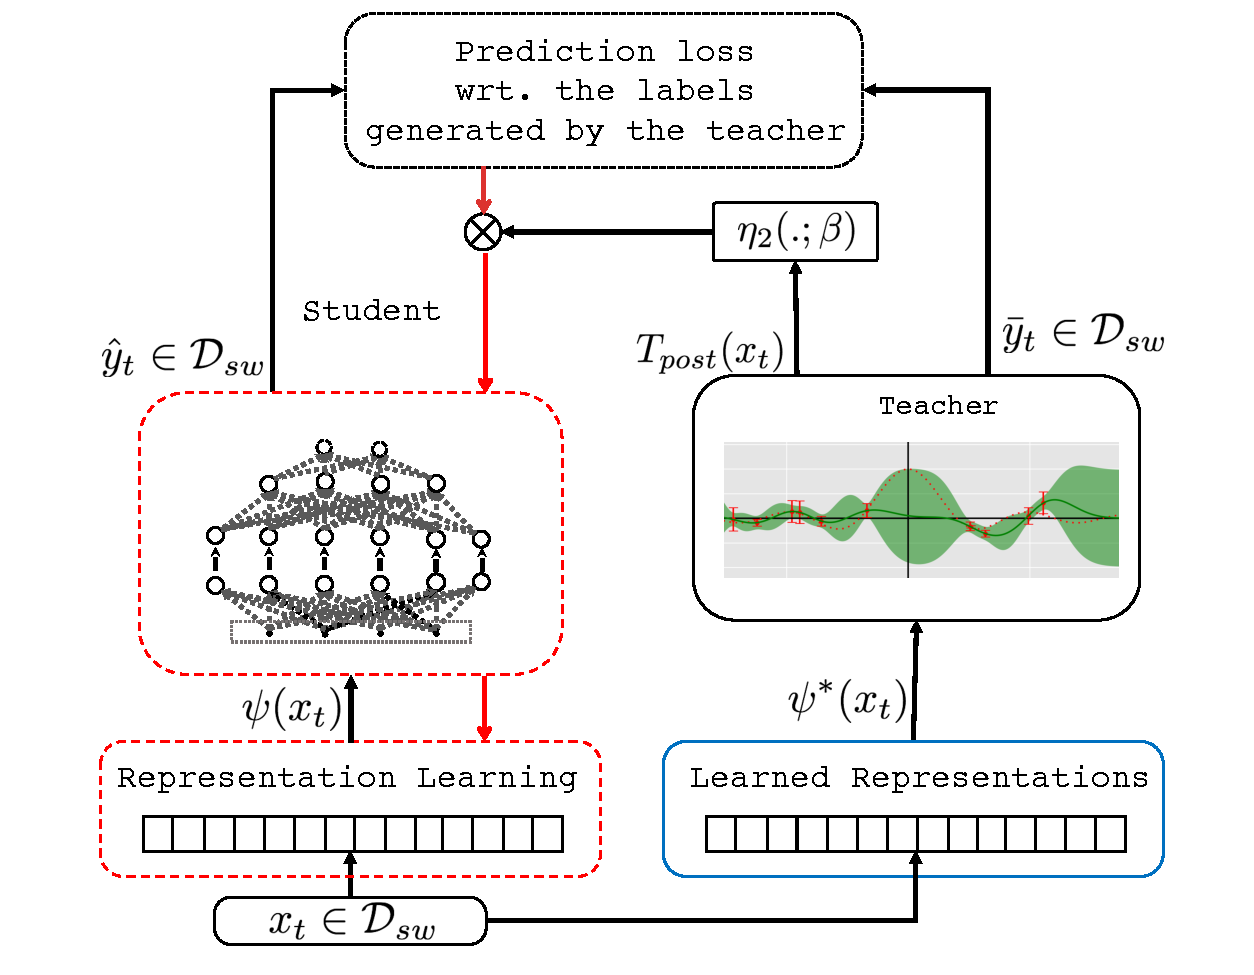
\includegraphics[width=\textwidth]{03-part-02/chapter-05/figs_and_tables/fig_fwl_step_3.pdf}
        \caption{\label{fig:step3}Step 3}
    \end{subfigure}%
    % }
    \caption{Illustration of \fwlfull: Step 1: Pre-train \std on weak data,  Step 2: Fit \tch to observations from the true function, and Step 3: Fine-tune \std on labels generated by \tch, taking the confidence into account. Red dotted borders and blue solid borders depict components with trainable and non-trainable parameters, respectively.}
    \label{fig:model_fwl}
\end{figure}